\documentclass[a4paper]{article}
\usepackage[a4paper,  margin=1.0in]{geometry}

\usepackage{graphicx}
\usepackage{float}
\usepackage{hyperref}
\usepackage{listings}
\lstset{
basicstyle=\small\ttfamily,
columns=flexible,
breaklines=true
}

\usepackage{polski}
\usepackage[utf8]{inputenc}
\begin{document}


\title{Ćwiczenie nr 4 z MBI, Analiza danych sekwencyjnych człowieka}
\author{Kinga Kimnes, Jakub Skałecki}
\maketitle

\section{Liczenie pokrycia}


W tej części ćwiczenia obliczono pokrycie przykładowych plików BAM paczki WES z odczytami pochodzącymi z niewielkiego fragmentu chromosomu 22. Jest dostępnych 46 plików BAM, przy czym każdy z nich to próbka otrzymana z sekwencjonowania tego samego kawałka chromosomu 22.

Zbadano pokrycie tych odczytów ze współrzędnymi regionów sekwencjonowanych metodą WES w projekcie 1000 Genomes. Posiadano 100 takich współrzędnych (początek i koniec). Fragment pliku \path{WES.1KG.WUGSC/extdata/chr22_400_to_500.bed}

\begin{verbatim}
  V1       V2       V3
  1: 22 21345867 21346168
  2: 22 21346453 21346708
  3: 22 21347033 21347243
  4: 22 21347901 21348093
\end{verbatim}

Otrzymano macierz pokrycia każdej próbki z każdym regionem, czyli macierz 100x46. Obliczono medianę pokrycia dla każdej próbki.

Największą medianę ma próbka \texttt{NA19137} i wynosi \texttt{76.03475}.
Najmniejszą medianę ma próbka \texttt{NA18991}, a jej wartość to \texttt{21.06271}.


\section{Wykrywanie zmian liczby kopii DNA przy użyciu narzędzia CODEX}

W ramach tej części wykorzystano przeliczone pokrycie dla 99 próbek z projektu 1000 Genomes dla chromosomu 20 (plik coverage). Wynik kontroli jakości:

\begin{verbatim}
Excluded 279 exons due to extreme coverage.
Excluded 18 exons due to extreme exonic length.
Excluded 22 exons due to extreme mappability.
Excluded 15 exons due to extreme GC content.
After taking union, excluded 318 out of 4702 exons in QC.
\end{verbatim}

W wyniku kontroli zostało usuniętych \texttt{318} eksonów.
Po zmianie parametrów progowych na $gc\_thresh\_from=25, gc\_thresh\_to=75)$ otrzymano następujące wyniki:

\begin{verbatim}
Excluded 279 exons due to extreme coverage.
Excluded 18 exons due to extreme exonic length.
Excluded 22 exons due to extreme mappability.
Excluded 88 exons due to extreme GC content.
After taking union, excluded 325 out of 4702 exons in QC.
\end{verbatim}

Zmieniła się zatem liczba wykluczonych eksonów - wykluczono ich \texttt{325}.

Przy użyciu narzędzia CODEX wykryto \texttt{440 zmian liczby kopii}. Wśród nich zawiera się \texttt{262 duplikacji} i \texttt{178 delecji}.
Występują \texttt{3 homozygotyczne delecje} (parametr copy\_no == 0) dla próbek \texttt{NA18486, NA18912 oraz NA18965}:
\footnotesize
\begin{verbatim}

   sample_name chr cnv    st_bp    ed_bp length_kb st_exon ed_exon raw_cov norm_cov copy_no lratio    mBIC targetCount
X.151     NA18486  20 del 56793551 56803479     9.929    3650    3652       0       21       0     21   0.683       2
X.345     NA18912  20 del 56793551 56803479     9.929    3650    3652       0       21       0     21   0.683       2
X.373     NA18965  20 del 61460052 61460361      0.31    4031    4032       0       22       0     22 380.372       1
\end{verbatim}
 \newpage
\begin{figure}[h]
    \centering
    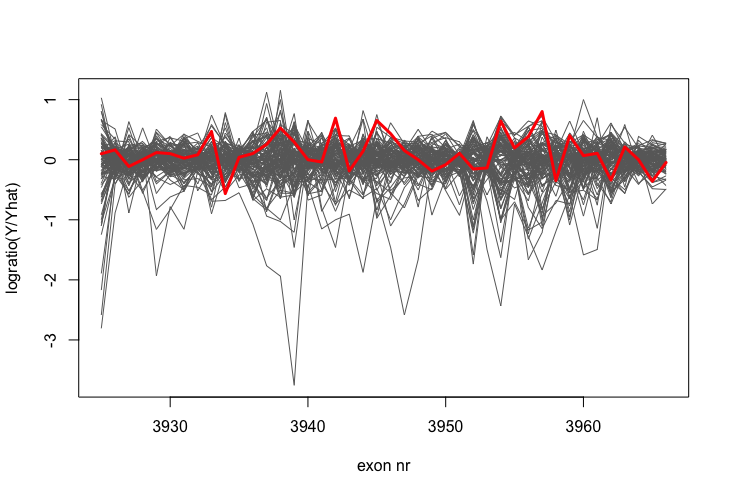
\includegraphics[width=1.0\textwidth]{plot_change_no_1.png}
    \label{fig:igv}
    \caption[]{Wykres sporządzony dla zmiany o numerze 1}
\end{figure}


\end{document}
